\section{引言}\label{ux5f15ux8a00}

眼底成像是早期眼科疾病辅助筛查的重要依据，能够反映视网膜、视盘、血管和黄斑区域的多类病变征象。通过对眼底成像进行分析，有助于患者发现潜在病变并尽早干预，从而降低不可逆的视力损伤甚至视力丧失的风险。随着眼科疾病筛查规模扩大，人工阅片面临阅片耗时、依赖专家经验和基层医疗资源不足等问题，因此基于眼底图像的智能辅助诊断具有重要应用价值\hyperref[_Ref213949315]{{[}1{]}}。围绕眼底图像智能诊断，现有方法大体可分为传统机器学习、视觉大语言模型和卷积神经网络三类路线。传统机器学习通常依赖图像增强、病灶分割、纹理或形态等人工特征，再结合支持向量机、随机森林等分类器完成识别\hyperref[_RefRahman2022MLFundus]{{[}2{]}}，这类方法具有一定可解释性，但特征设计依赖先验经验，对复杂眼底病灶和多疾病共存场景的表达能力有限。近年来，视觉大语言模型和医学多模态模型为眼科图像理解、图文联合分析和医学报告生成提供了新的研究方向\hyperref[_RefLim2024VLVOphthalmology]{{[}3{]}}\hyperref[_RefUrooj2025LLMMedicalImage]{{[}4{]}}，但其训练和微调通常依赖大规模高质量标注数据、图文配对数据以及较高算力资源，在医疗数据稀缺、隐私受限和临床部署资源有限的场景中仍面临较高成本。相比之下，以CNN为代表的深度视觉模型能够直接从眼底图像中学习局部纹理、病灶区域和空间结构特征，已广泛应用于疾病分类\hyperref[_Ref213871637]{{[}5{]}}、病灶分割\hyperref[_Ref213948625]{{[}6{]}}、医学图像重建\hyperref[_Ref213948898]{{[}7{]}}和疾病诊断与预测\hyperref[_Ref213949262]{{[}8{]}}等任务。因此，本文选择CNN作为多标签眼科疾病识别任务的基础路线。然而，在真实临床部署中，基于CNN的眼底疾病识别方法仍面临多标签疾病共存、跨机构部署泛化性能下降以及医疗数据隐私保护等挑战。具体而言：

1.在临床眼底疾病识别中，单眼可能同时存在多种疾病，若仍采用标准单标签分类器或将不同疾病完全独立建模，容易造成误判和漏检\hyperref[_Ref213949362]{{[}9{]}}。近年来，自然图像中也存在多标签识别方法的相关工作，比如ML-GCN \hyperref[_Ref213949382]{{[}10{]}}，通过统计各标签出现的频率建立图关联性，使得识别出某个标签后，更有可能识别出其关联标签，从而减少漏检。而在眼底多标签疾病识别中，各疾病之间的关联性更加错综复杂，仅靠标签频率来建立疾病关联性的方法对于这种复杂情况效果可能不可靠。因此，面向眼底多疾病共存场景，仍需要探索一种更高效可靠的疾病标签与图像特征关联构建方法。

2.医疗图像数据与自然图像不同，其标注通常需要专业医生完成，数据获取和标注成本较高；同时，不同医疗机构之间还存在数据共享限制、标签空间不统一等问题，使多源域数据的访问与协同训练并不总是容易实现。然而，即使通过某个医疗机构的源域数据集训练得到了一个性能良好的模型，将其应用到另外的机构时，目标域数据也常因成像设备、光照条件和人工处理流程差异产生域偏移\hyperref[_Ref213949348]{{[}11{]}}，导致模型性能下滑。如\figsubref{fig:intro-domain-gap}{a1}和\figsubref{fig:intro-domain-gap}{a3}所示，源域和目标域的分布有差异，仅在源域训练的基线模型（\figsubref{fig:intro-domain-gap}{b1}）得到的决策边界可能不适用于目标域分布（\figsubref{fig:intro-domain-gap}{b2}）。常见的域适应方法DA选择将源域和目标域数据一同送入模型训练来对齐域分布\hyperref[_Ref213949354]{{[}12{]}}，但这需要训练阶段访问目标域数据；多源域泛化方法虽可避免访问目标域，但通常依赖多个源域共同训练。在医疗数据协同训练受限的实际场景中，上述前提往往难以满足。因此，探索仅利用单一源域学习可迁移疾病相关表示的单域泛化方法，更符合跨机构部署需求。

\begin{figure}[!htb]
\centering
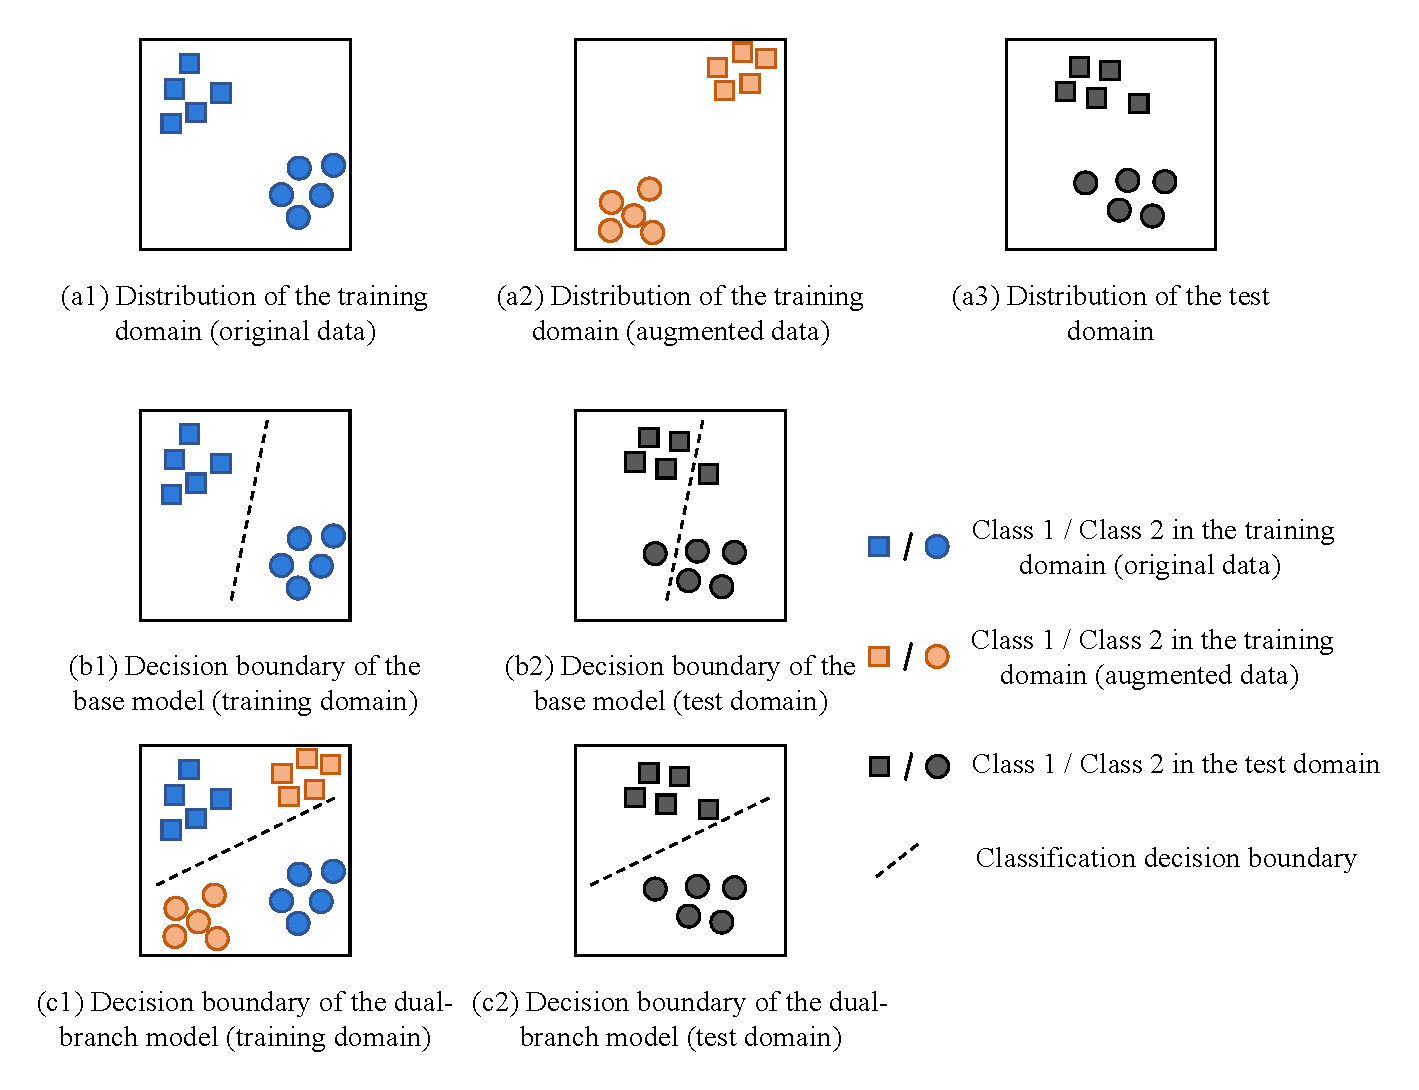
\includegraphics[width=0.72\textwidth]{./images/media/image1_padded.pdf}
\caption{常规模型与双分支模型的决策边界示意图}
\label{fig:intro-domain-gap}
\end{figure}

3.医疗数据比起自然图像更加敏感，存在更高的数据隐私风险，且在传统域适应跨域场景下更为突出。常见的攻击方法可以通过模型的训练梯度逆向恢复出患者的数据\hyperref[_Ref213949393]{{[}13{]}}。针对此问题，目前已有联邦学习、同态加密、安全多方计算和差分隐私等隐私保护方法研究，但是隐私保护与模型性能之间通常存在权衡关系；尤其在DA场景中，源域和目标域数据需要同时参与训练，可能带来隐私机制添加复杂、多域性能衰减明显等问题。因此，需要在单域泛化训练流程中进一步探索隐私保护与跨域性能之间的平衡方法。

为应对上述三个关键挑战，我们构建了一个融合隐私保护的多标签眼科疾病识别可解释单域泛化框架。针对眼科场景中普遍存在的多疾病共存问题，我们引入基于 Transformer 的自适应标签-特征关联性构建模块，通过自注意力建模标签间的内在关联关系，并利用交叉注意力将标签语义与对应的图像特征进行融合，在标签层面与特征层面同时构建疾病共现依赖，从而减少多标签识别中的误检与漏检；针对多机构数据访问受限与跨机构部署域偏移并存的问题，我们提出双分支引导的域不变特征提取模块，仅利用单一源域数据进行训练，通过对训练域原始图像及其分布扰动后的增强图像构建双分支结构（如\figsubref{fig:intro-domain-gap}{a1}和\figsubref{fig:intro-domain-gap}{a2}所示），在特征层面挖掘两者的共性表示。同时，引入基于 CAM 的类别关注区域作为先验引导，促使模型聚焦于疾病相关区域，从而抑制域特定噪声特征的学习，使得模型能够形成更适用于未知域分布的决策边界（\figsubref{fig:intro-domain-gap}{c1}），并在未知测试域上保持稳定的分类性能（\figsubref{fig:intro-domain-gap}{c2}）。此外，CAM 热图还为模型预测提供了直观的关注区域可视化，增强了模型的可解释性；针对跨域医疗场景下的数据隐私风险，本文在单域泛化训练过程中集成自适应高斯差分隐私机制，通过在梯度更新阶段注入噪声实现隐私保护。在中等隐私预算条件下，该机制能够在不显著牺牲模型性能的前提下提供有效的隐私保障，实现跨域泛化能力与数据隐私保护的兼顾。

最后在多个具有代表性的眼底影像数据集和跨站点测试设置上进行的系统实验表明，该框架在保持良好可解释性的同时，在跨域多标签分类性能与隐私约束条件下均展现出稳定且优越的表现。

我们的贡献如下：

\begin{sloppypar}
1.提出了一种自适应标签-特征关联性构建模块（Adaptive label-feature relevance construction, ARC），基于 Transformer 的自注意力与交叉注意力机制，在标签层面与特征层面同时建模疾病共现依赖，有效降低了多标签眼科疾病识别中的误检与漏检问题。

2.设计了一种双分支引导域不变特征提取模块（Dual-branch guided domain invariant feature extraction, DFE）。该模块面向多机构数据难联合训练与跨机构部署域偏移并存的场景，通过分布扰动增强与类别激活映射（CAM）联合引导，仅利用单一源域学习可迁移的疾病相关表示，不仅提升了未知域泛化性能，同时增强了模型预测的可解释性。

3.将自适应高斯差分隐私机制（Adaptive Gaussian differential privacy, AdaGDP）集成至单域泛化训练流程中，在不引入目标域数据的前提下，实现了隐私保护与跨域泛化性能之间的有效平衡，验证了在中等隐私预算条件下模型性能仍可接近非隐私基线。
\end{sloppypar}

本文的其余部分安排如下：第二节介绍了近年来的相关工作。所提出方法的具体阐述于第三节介绍，第四节展示完整的实验设置和结果。第五节得出结论并展开未来工作的讨论。
